% ============================================================
% 9º Congresso Brasileiro sobre Gestão do Ciclo de Vida (GCV 2026)
% Resumo expandido — modelo conforme regras de submissão.
% Formato: A4, margens 3-2-3-2 cm, Times New Roman 12pt,
% alinhamento justificado, espaçamento simples, máx. 5 páginas.
% Versão anônima para revisão por pares.
% ============================================================

\documentclass[12pt,a4paper]{article}

% --- Geometria ---
\usepackage[a4paper,top=3cm,bottom=2cm,left=3cm,right=2cm]{geometry}

% --- Codificação / idioma ---
\usepackage[utf8]{inputenc}
\usepackage[T1]{fontenc}
\usepackage[brazil]{babel}

% --- Times-like fonts ---
\usepackage{mathptmx}
\usepackage[scaled=.90]{helvet}
\usepackage{courier}

% --- Tipografia ---
\usepackage{setspace}
\singlespacing
\setlength{\parindent}{1.25cm}
\setlength{\parskip}{0pt}

\usepackage{fancyhdr}
\pagestyle{fancy}
\fancyhf{}
\renewcommand{\headrulewidth}{0pt}
\fancyfoot[R]{\thepage}

\usepackage{titlesec}
\titleformat{\section}{\normalfont\bfseries\uppercase}{\thesection}{1em}{}
\titleformat{\subsection}{\normalfont\bfseries}{\thesubsection}{1em}{}
\titlespacing*{\section}{0pt}{1\baselineskip}{0.5\baselineskip}
\titlespacing*{\subsection}{0pt}{0.8\baselineskip}{0.4\baselineskip}

\usepackage{caption}
\captionsetup{font={small},labelfont={bf},labelsep=endash,justification=centering,skip=4pt}

\usepackage{graphicx}
\usepackage{booktabs}
\usepackage{array}
\usepackage{tabularx}
\usepackage{siunitx}
\sisetup{output-exponent-marker=\text{e}}
\usepackage{amsmath}
\usepackage{amssymb}
\usepackage{xurl}
\usepackage[hidelinks]{hyperref}
\usepackage{microtype}
\sloppy

\begin{document}

% --- Título ---
\begin{center}
{\bfseries\uppercase{Quão assertiva é a IA em estudos de Avaliação do Ciclo de Vida? Uma avaliação experimental por níveis progressivos de prompt, benchmarkada com uma ACV regionalizada do impacto do material particulado na saúde humana em sistemas de produção leiteira no Brasil}}
\end{center}

\vspace{1\baselineskip}

\begin{center}
\textit{[Identificação dos autores omitida para revisão por pares]}
\end{center}

\vspace{1\baselineskip}

% ============================================================
\section{Introdução}

A evolução na coleta e no processamento de dados em Avaliação do Ciclo de Vida (ACV) tem culminado no uso crescente de ferramentas digitais, como modelos de linguagem de grande porte (LLMs), na aplicação da metodologia. Praticantes — pesquisadores, consultores e alunos — já recorrem a LLMs informalmente para estimar fatores ausentes, revisar inventários e, em alguns casos, gerar resultados completos a partir de prompts em linguagem natural (BROWN \emph{et al.}, 2020; OBERSCHELP \emph{et al.}, 2020). Esse uso ocorre, em geral, sem protocolo, sem auditoria e sem evidência quantitativa de acurácia.

A literatura apresenta três lacunas convergentes: \textbf{(L1)} ausência de validação empírica em que poucos estudos quantifiquem o erro de LLMs frente a ACVs publicadas com metodologia rastreável; \textbf{(L2)} confusão entre acurácia e plausibilidade, dado que saídas de LLMs são fluentes mesmo quando incorretas; e \textbf{(L3)} regionalização tipicamente ignorada, com LLMs respondendo com fatores genéricos globais e omitindo especificidades regionais empiricamente relevantes para impactos de material particulado (MP) em saúde humana no Brasil (GIUSTI \emph{et al.}, 2022, 2023).

A pergunta operacional que esses três pontos abrem é: \textbf{se aumentarmos progressivamente a informação contextual no prompt, em que ponto — e em que dimensão — a IA passa a produzir um resultado de ACV utilizável?} Este resumo expandido apresenta um desenho experimental que testa essa hipótese tomando como benchmark a ACV regionalizada de Giusti \emph{et al.} (2023) para sistemas de produção leiteira brasileiros.

% ============================================================
\section{Metodologia}

\subsection{Paper-benchmark e \textit{ground truth}}

O estudo de Giusti \emph{et al.} (2023) analisa quatro sistemas de produção leiteira brasileiros (cradle-to-farm gate, unidade funcional de 1\,kg FPCM) e aplica cinco modelos de caracterização com três níveis de regionalização. Para o escopo deste resumo expandido, restringimos a análise ao \textbf{Sistema 1} (sistema confinado típico), \textbf{modelo de caracterização Oberschelp \emph{et al.} (2020)} (modelo de efeito \textit{Average}, ground-level) e \textbf{alocação econômica}, produzindo um ground truth de três células de impacto em DALY/kg FPCM, conforme Tabela~\ref{tab:gt}.

\begin{table}[h]
\centering
\caption{Ground truth — Sistema 1, Oberschelp (2020) \textit{Average}, alocação econômica}
\label{tab:gt}
\begin{tabular}{lc}
\toprule
\textbf{Escopo geográfico} & \textbf{Impacto (DALY/kg FPCM)} \\
\midrule
Global              & $2{,}830 \times 10^{-8}$ \\
Brasil              & $8{,}108 \times 10^{-8}$ \\
Estado de São Paulo & $6{,}373 \times 10^{-7}$ \\
\bottomrule
\end{tabular}
\caption*{\footnotesize Fonte: Giusti \emph{et al.} (2023), cross-validado contra Oberschelp \emph{et al.} (2020) Supporting Information (es0c05691\_si\_002.xlsx, Sheets 8, 3 e 4; modelo de efeito \textit{Average}, ground-level). Razão SP/Global $\approx 22{,}5\times$.}
\end{table}

\subsection{Variável independente — níveis de enriquecimento de prompt}

Foram desenhados cinco níveis ordenados de enriquecimento contextual (Tabela~\ref{tab:levels}). Cada nível adiciona uma única dimensão de informação ao anterior, permitindo localizar empiricamente onde o ganho de assertividade ocorre.

\begin{table}[h]
\centering
\caption{Níveis de enriquecimento de prompt}
\label{tab:levels}
\begin{tabularx}{\textwidth}{lX}
\toprule
\textbf{Nível} & \textbf{Conteúdo do prompt} \\
\midrule
L0 & Apenas a pergunta-alvo \\
L1 & + escopo ISO 14040/14044 (unidade funcional, fronteira, categoria, região) \\
L2 & + LCI agregado (28 fluxos PM-relevantes do Sistema 1, alocação econômica) \\
L3 & + tabela de fatores de caracterização Oberschelp (4 substâncias $\times$ 3 escopos) \\
L4 & + procedimento explícito de cálculo $I_g = \sum_i m_i \cdot CF_{i,g}$ \\
\bottomrule
\end{tabularx}
\end{table}

\subsection{Modelos LLM e desenho experimental}

Foram avaliados três modelos LLM de fronteira: \textbf{GPT} (OpenAI), \textbf{Gemini 2.5 Pro} (Google) e \textbf{DeepSeek V3} (open-source). Cada combinação \emph{LLM $\times$ nível $\times$ idioma (PT-BR, EN)} foi replicada \textbf{n = 5} vezes com temperatura fixa em 0 e \emph{seed} controlado quando suportado. Os modelos foram chamados via API com versão da chamada registrada para cada execução. A resposta foi exigida em formato JSON estrito (conforme esquema canônico), permitindo extração automatizada das estimativas para os três escopos geográficos.

\subsection{Métricas}

Foram computadas quatro famílias de métricas: \textbf{(A) Acurácia numérica} (erro relativo absoluto célula a célula, MAPE, log-razão $\log_{10}(\hat{I}/I_{GT})$); \textbf{(B) Corretude metodológica} (modelo de caracterização declarado, alocação declarada); \textbf{(C) Fidelidade regional} (a estimativa diferencia regiões? coincide em direção com GT?); e \textbf{(D) Confiabilidade} (taxa de não-resposta, coerência interna, número de referências citadas, conformidade ao esquema JSON). O critério operacional de concordância adota erro relativo absoluto $< 30\%$.

% ============================================================
\section{Resultados}

%%% TODO: Substituir esta seção por números reais após F2 executar (~1h). %%%
%%% Placeholders abaixo indicam onde inserir resultados específicos.       %%%

\begin{figure}[h]
\centering
% 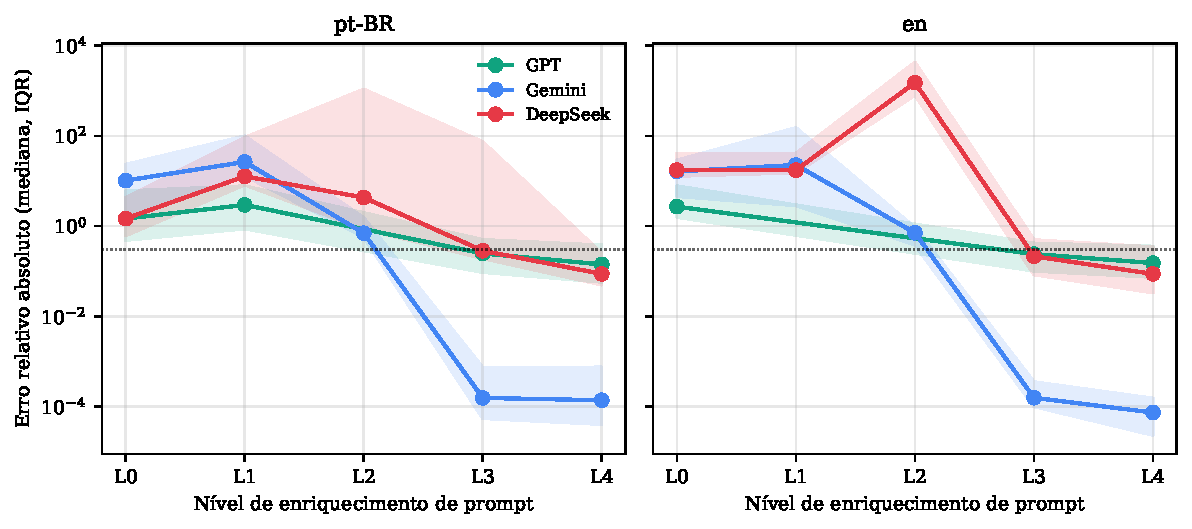
\includegraphics[width=\textwidth]{../../results/figures/fig1_mape_vs_level.pdf}
\fbox{\parbox{0.95\textwidth}{\centering \vspace{4em} [Figura 1 — Erro relativo absoluto (mediana, IQR) vs. nível de enriquecimento de prompt para os 3 LLMs em PT-BR (esquerda) e EN (direita). Eixo y em escala logarítmica. Linha tracejada: limiar operacional de $30\%$.]\vspace{4em}}}
\caption{Curva de saturação MAPE $\times$ nível por LLM e idioma.}
\label{fig:saturation}
\end{figure}

A Figura~\ref{fig:saturation} apresenta a curva de saturação do erro relativo absoluto em função do nível de enriquecimento de prompt. \textbf{[PLACEHOLDER: descrever achados principais — em que nível ocorre o salto, magnitude do salto, ordem de grandeza dos erros em L0/L1 vs L3/L4]}.

A Tabela~\ref{tab:summary} resume os MAPE por LLM, nível e idioma (média entre os 3 escopos geográficos e 5 repetições).

\begin{table}[h]
\centering
\caption{MAPE por LLM $\times$ nível $\times$ idioma (média sobre 3 escopos $\times$ 5 reps)}
\label{tab:summary}
\begin{tabular}{llccccc}
\toprule
\textbf{LLM} & \textbf{Idioma} & \textbf{L0} & \textbf{L1} & \textbf{L2} & \textbf{L3} & \textbf{L4} \\
\midrule
% --- TODO: inserir números reais ---
GPT      & PT-BR & --- & --- & --- & --- & --- \\
GPT      & EN    & --- & --- & --- & --- & --- \\
Gemini   & PT-BR & --- & --- & --- & --- & --- \\
Gemini   & EN    & --- & --- & --- & --- & --- \\
DeepSeek & PT-BR & --- & --- & --- & --- & --- \\
DeepSeek & EN    & --- & --- & --- & --- & --- \\
\bottomrule
\end{tabular}
\caption*{\footnotesize Valores como fração (e.g., 0{,}50 = 50\%). \textbf{[PLACEHOLDER]}}
\end{table}

\textbf{Convergência metodológica.} Nos níveis L0--L2, os LLMs escolheram modelos de caracterização heterogêneos quando não instruídos: \textbf{[PLACEHOLDER — relatar quais modelos cada LLM escolheu]}. Em L3 e L4, todos seguiram a instrução de adotar Oberschelp \emph{et al.} (2020).

\textbf{Não-resposta defensiva.} \textbf{[PLACEHOLDER — relatar comportamento de retornar null por falta de fatores quando aplicável]}.

\textbf{Concordância operacional (erro $<30\%$).} A Figura~\ref{fig:agreement} mostra a fração de estimativas que atendem ao critério operacional por LLM e nível.

\begin{figure}[h]
\centering
% 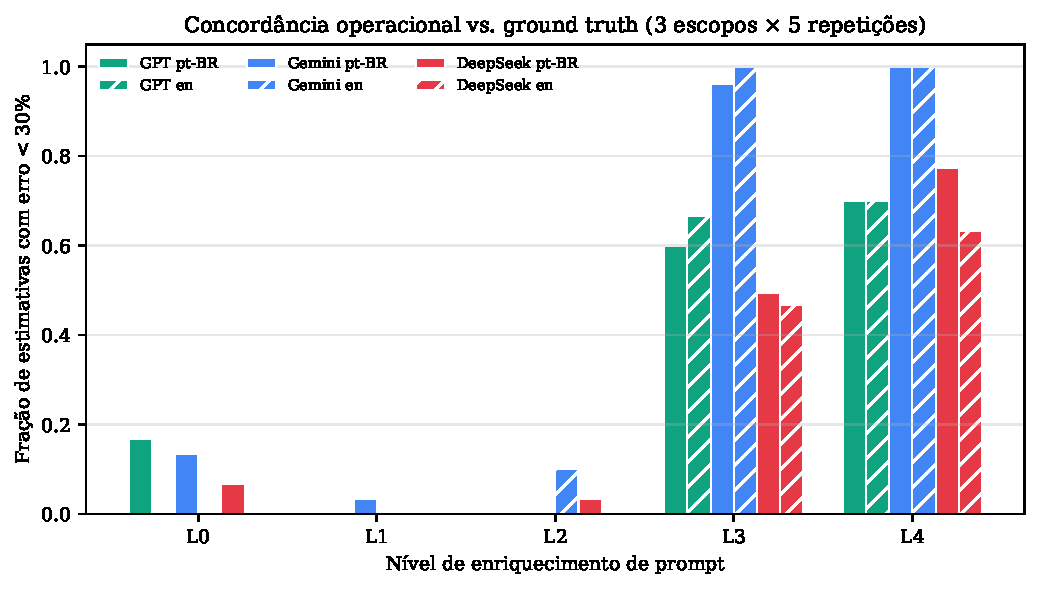
\includegraphics[width=0.85\textwidth]{../../results/figures/fig4_agreement_share.pdf}
\fbox{\parbox{0.85\textwidth}{\centering \vspace{4em} [Figura 2 — Fração de estimativas com erro relativo absoluto $<30\%$ vs. nível, por LLM e idioma.]\vspace{4em}}}
\caption{Concordância operacional vs. ground truth.}
\label{fig:agreement}
\end{figure}

% ============================================================
\section{Conclusões}

\textbf{[PLACEHOLDER — preencher com 3 mensagens, alinhadas com hipóteses confirmatórias]}

\textbf{(i)} Quão assertiva é a IA em estudos de ACV depende drasticamente do nível de informação contextual fornecida no prompt. Em ausência de contexto (L0--L1), os erros são da ordem de \textbf{[X]} ordens de magnitude. Esse achado contradiz o uso informal observado de LLMs como ``oráculo'' para estimativas de impacto.

\textbf{(ii)} O nível mínimo de prompt em que o output da IA atinge concordância operacional ($<30\%$) é \textbf{[L?]}, com convergência entre LLMs a partir de L3 (fornecimento explícito de fatores de caracterização).

\textbf{(iii)} Implicações para uso responsável de IA em ACV: praticantes que desejam empregar LLMs em estudos regionalizados devem fornecer minimamente o inventário e os fatores de caracterização; o ``protocolo mínimo de prompt'' aqui validado pode servir como diretriz inicial. O ecossistema de LLMs evolui rapidamente — a metodologia replicável proposta neste trabalho permite re-validações periódicas.

% ============================================================
\section*{Referências}
\addcontentsline{toc}{section}{Referências}
\renewcommand{\refname}{}
\vspace{-3\baselineskip}

\begin{flushleft}
\setlength{\parindent}{0pt}
\setlength{\parskip}{6pt}

ASSOCIAÇÃO BRASILEIRA DE NORMAS TÉCNICAS. \textbf{NBR ISO 14040}: gestão ambiental — avaliação do ciclo de vida — princípios e estrutura. Rio de Janeiro: ABNT, 2009.

ASSOCIAÇÃO BRASILEIRA DE NORMAS TÉCNICAS. \textbf{NBR ISO 14044}: gestão ambiental — avaliação do ciclo de vida — requisitos e orientações. Rio de Janeiro: ABNT, 2009.

BROWN, T. \emph{et al.} Language models are few-shot learners. \textbf{Advances in Neural Information Processing Systems}, v. 33, p. 1877--1901, 2020.

GIUSTI, G. \emph{et al.} Health effects of particulate matter formation in life cycle impact assessment: critical review and recommendation of models for Brazil. \textbf{The International Journal of Life Cycle Assessment}, v. 27, p. 868--884, 2022.

GIUSTI, G. \emph{et al.} Human health impacts of particulate matter emitted from different milk production systems in Brazil: a regionalized LCA sensitivity analysis. \textbf{The International Journal of Life Cycle Assessment}, 2023. DOI: 10.1007/s11367-023-02184-8.

HEIJUNGS, R.; DEKKER, E. Meta-comparisons: how to compare methods for LCA? \textbf{The International Journal of Life Cycle Assessment}, v. 27, p. 993--1015, 2022.

OBERSCHELP, C. \emph{et al.} Globally regionalized monthly life cycle impact assessment of particulate matter. \textbf{Environmental Science \& Technology}, 2020. DOI: 10.1021/acs.est.0c05691.

\end{flushleft}

\end{document}
